\documentclass{beamer}
%\documentclass[trans]{beamer} %om te printen!
%\transglitter etc: kunt ge pas zien op Full Screen (Ctrl+L)

\usepackage{graphicx,multicol}
\usepackage[all]{xy}
\usepackage{beamerouterthememiniframes, beamercolorthemeann,srcltx,hyperref}

\setbeamercolor{normal text}{fg=black!70}
\setbeamertemplate{navigation symbols}{}%geen navigatie
\setbeamertemplate{blocks}[rounded][shadow=true]


\title{Performance Analysis of a Real-Time Video Processing System}
\author{Frank Vanbever}
\date{27 January 2014}

\begin{document}

\begin{frame}[plain]

\includegraphics[width=0.4\paperwidth]{VUB_logo.jpg}
\vspace{2cm}
\titlepage
\end{frame}


%\section[Overzicht]{}%rechte haken dienen om niet in de outline te komen
%maar wel vanboven in het donkergroene balkje

%\begin{frame}[plain]{Outline}
%\end{frame}
%
%\begin{frame}[plain]{Outline}
%\tableofcontents[pausesections]
%\end{frame}
%
%
%\section{blabla}
%
%\begin{frame}
%\begin{alertblock}{}
%\begin{center}
%blabla
%\end{center}
%\end{alertblock}
%\end{frame}


\section{Table of Contents}


\begin{frame}{Contents}
  \begin{itemize}
  \item Introduction
  \item Platform Overview
    \begin{itemize}
    \item Zynq-7000
    \item ZC-702 Base TRD
    \end{itemize}
  \item High Level Synthesis
    \begin{itemize}
    \item Vivado HLS
    \end{itemize}
  \item Performance Analysis
    \begin{itemize}
    \item Roofline Model
    \item Memory Architecture
    \item Directives
    \item Resource Consumption
    \item Memory Bandwidth
    \end{itemize}
  \end{itemize}
\end{frame}

\section{Introduction}

\begin{frame}{Introduction}
  \begin{itemize}
  \item Until recently computing performance could be gained
    maintaining the sequential programming paradigm
    \begin{itemize}
    \item Primarily through Moore's law
    \item multiple-issue, pipelining and \emph{out-of-order} execution
      perpetuated this
    \end{itemize}
  \item Eventually a \emph{power wall} was hit. The size of MOSFETs
    couldn't keep on decreasing whilst the frequency decreased.
  \item The solution was to turn to parallel processors, containing
    more than one processing unit working at a time.
    \begin{itemize}
    \item This caused a new problem: How could this parallel hardware
      be used efficiently.
    \item A new programming paradigm is necessary
    \end{itemize}
  \end{itemize}
\end{frame}

% \begin{frame}{Processing Components}
%   \begin{itemize}
%   \item Three types of computing components saw widespread use
%     \begin{itemize}
%     \item \textbf{Multicore Processors}
%       \begin{itemize}
%       \item Solution presented by traditional manufacturers
%       \item Multiple CPU cores on the same die.
%       \item Easiest to program, modest parallelism
%       \end{itemize}
%     \item \textbf{Graphics Processing Units}
%       \begin{itemize}
%       \item Originally used as graphics coprocessor in traditional
%         computers
%       \item Many multithreaded SIMD cores
%       \item Programmed using OpenCL or CUDA, best floating-point
%         performance, bad conditional execution performance
%       \end{itemize}
%     \item \textbf{Field Programmable Gate Array}
%       \begin{itemize}
%       \item Devices containing a vast amount of configurable logic
%         connected through programmable connections
%       \item Unconstrained by \emph{Von Neuman}, use dataflow paradigm
%       \item Typically programmed using VHDL or Verilog, poor
%         floating-point performance
%       \end{itemize}
%     \end{itemize}
%   \end{itemize}
% \end{frame}

\section{Platform Overview}

\begin{frame}{Zynq-7000}
  \begin{itemize}
  \item The Zynq-7000 is a \emph{System On Chip} or SoC which consists
    of a dual core ARM Cortex-A9 and Xilinx programmable logic
    \begin{itemize}
    \item These are called the Processing System (PS) and Programmable
      Logic (PL)
    \end{itemize}
  \item The processing system consists of the Application Processor
    Unit (APU), a memory controller and numerous I/O peripherals
  \item The Programmable Logic is based on Artix-7 or Kintex-7
    technology dependent on the type
  \end{itemize}
\end{frame}

\begin{frame}{Interconnect}
  \begin{itemize}
  \item The interconnections in the Zynq SoC use the Advanced
    Extensible Interface (AXI) protocol which is part of ARM's
    Advanced Microcontroller Bus Architecture (AMBA) v3.0
  \item The interconnections between the PS and PL play an important
    role in the system's performance
  \item \textbf{AXI\_HP} The system has four \textbf{H}igh
    \textbf{P}erformance interconnections connecting PL masters to DDR
    and OCM memories using double FIFO buffers
  \item \textbf{AXI\_GP} The system has four \textbf{G}eneral
    \textbf{P}urpose ports divided into 2 master ports and 2 slave
    ports.
  \item \textbf{AXI\_ACP} The \textbf{A}ccelerator \textbf{C}oherency
    \textbf{P}ort connects the PL directly with the APU caches through
    the Snoop Control Unit with optional coherency
  \end{itemize}
\end{frame}

\begin{frame}{Base Targeted Reference Design 14.5}
  \begin{itemize}
  \item A preexisting system was used as the base for the experiments
  \item On the hardware side it consists of a complete image
    processing pipeline
    \begin{itemize}
    \item This pipeline can be split into 3 stages, reading and
      writing to/from memory, each using their own DMA controller
    \end{itemize}
  \item The software side consists of a bootloader, the Xilinx Linux
    Kernel and a number of applications
  \item The goal of this system is to apply the Sobel operator to the video in real-time
  \end{itemize}
\end{frame}

\section{High Level Synthesis}

\begin{frame}{High Level Synthesis}
  \begin{itemize}
  \item A recurring theme is the relative difficulty of implementing
    an algorithm on FPGA
    \begin{itemize}
    \item Both development and synthesis take considerably longer
    \end{itemize}
  \item HLS tools partially alleviate these problems
    \begin{itemize}
    \item Typically a C,C++ or SystemC program is converted into VHDL
      or Verilog
    \item This improves programmer productivity
    \end{itemi
ze}

  \item Vivado HLS was used for this thesis
    \begin{itemize}
    \item C code is compilable allowing pre-synthesis verification
      testbenches, which in turn can be compiled to SystemC for
      post-synthesis verification
    \item A multitude of optimizations and interfaces are available
    \item Synthesis reports and analysis perspective contains information about timing, latency and resource consumption
    \end{itemize}
  \end{itemize}
\end{frame}

\section{Performance Analysis}

\begin{frame}{Roofline Model}
  
  \begin{itemize}
  \item The roofline model is a visial model that gives insight into
    factors influencing performance
    \begin{itemize}
    \item It is based on the observation that bandwidth is the
      constraining resource on system performance
    \item The model is a plot of the peak computational performance as
      a function of the computational performance
    \end{itemize}
  \end{itemize}
  \begin{figure}[H]
    \centering
    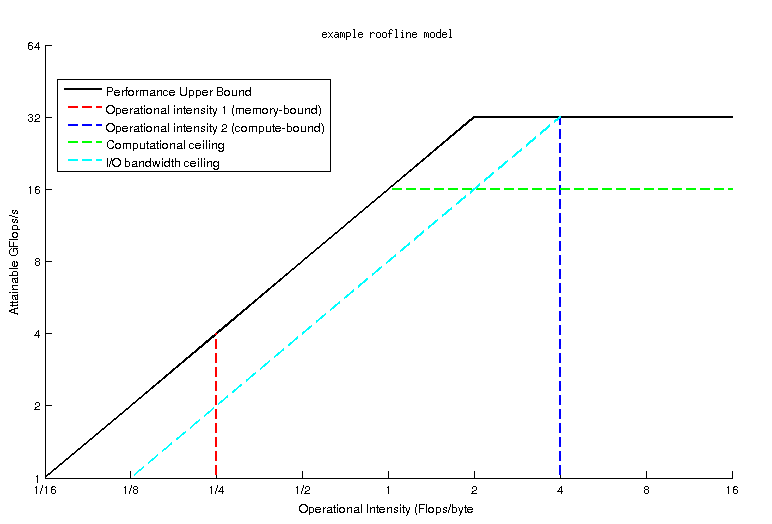
\includegraphics[scale=0.3]{../images/matlab_plots/roofline_example.png}

  \end{figure}
\end{frame}


\begin{frame}{Memory Architecture}
  \begin{itemize}
  \item Buffers influence the computational intensity, 2 types are
    used
    \begin{itemize}
    \item \textbf{Linebuffers} buffer a number of lines of the
      application, in this case 3. Implemented as BRAMS for their dual
      port nature
    \item \textbf{Memory Windows} buffer the values on which the Sobel
      operation is applied. Implemented as registers to give
      instantaneous access to all values at the same time
    \end{itemize}
  \item The implementation reads and writes one 32 bpp pixel every
    iteration. The sobel operator get applied 3 times giving following
    expression for the CI \medskip
    \begin{center}
      $CI\;=\;\frac{3 \times (H \times W)}{4 \times 2 \times (H \times
        W)} = \frac{3}{8}$
    \end{center}
  \end{itemize}
\end{frame}

\begin{frame}{Directives}
  \begin{itemize}
  \item The impact of directives following on the system's performance
    was tested and compared to the original configuration
    \begin{itemize}
    \item \textbf{Pipelining} allows for the concurrent execution of
      the operations in the algorithm. After the initial latency a new
      output can be written after II cycles
    \item \textbf{Loop Flattening} is a loop level optimization that
      combines nested loops into 1 loop. Disabling it prevents timing
      violations and increased initiation interval
    \item \textbf{Dependence} provides the compiler with extra
      information on the intra- or inter-dependencies in the
      code. Notifying the compiler of a mistakenly identified
      dependency accessing the linebuffer removes the need for an extra
      cycle
    \end{itemize}
  \item Only 2 configurations were found to satisfy the system
    constraints.
  \end{itemize}

\end{frame}
\begin{frame}{Resource Consumption \& Memory Bandwidth}
  \begin{itemize}
  \item The resource consumption determines the scalability of the system. In the case of the TRD the AXI HP interfaces were found to be the constraining factor allowing 3 possible instances
  \item As more AXI HP interfaces are used the available bandwidth increases
    \begin{itemize}
    \item Only using 4 interfaces the DDR RAM bandwidth becomes the constraining factor
    \end{itemize}
    \item In the case of the TRD the throughput remains constrained by the core 
  \end{itemize}
\end{frame}



\section{Conclusion}

\begin{frame}{Conclusion}
  \begin{itemize}
  \item The performance of a Zynq based system is influenced by a number of factors
    \begin{itemize}
    \item The memory implementation influences the Computational Intensity
    \item The number and type of AXI interconnects used play a decisive role in the bandwidth
    \end{itemize}
  \item HLS synthesis tools present a serious productivity improvement
  \item The necessary DMA controllers impact the available resources
  \end{itemize}
The Zynq platform presents an interesting hybrid between an FPGA and a CPU, especially when considered in an embedded systems context.
\end{frame}


\end{document}
